\chapter{Transformaties combineren}
\label{hoofdstuk:ETT}

In dit hoofdstuk worden twee algoritmes behandeld die varianten zijn van elkaar. Beide algoritmes transformeren een gegeven muziekstuk tot een nieuw muziekstuk zodat dat de totale consonantiescore zo hoog mogelijk is. Dit gebeurt door een aantal toegelaten operaties op het oorspronkelijke muziekstuk. Buiten de originele melodielijn zullen ook een aantal verschillende transformaties (zoals die beschreven zijn in onderdeel \ref{MT:afstand_vorige}) meegegeven worden aan het algoritme. Deze transformaties zullen door het algoritme gebruikt mogen worden om het originele stuk te transformeren naar een nieuw stuk met een hogere consonantiescore (De score die gebruikt wordt, is deze beschreven in onderdeel \ref{OBM:RPK}, volgens het `RPK-Model').

Voor elke noot van de melodielijn heeft het algoritme de keuze om ofwel de noot te behouden, ofwel deze te transformeren conform een van de transformaties die meegegeven werd aan het algoritme. Dit algoritme wordt beschreven in onderdeel \ref{ETT:algo1}. 

In gedeelte \ref{ETT:algo2} wordt een algoritme beschreven dat hetzelfde doel heeft maar voldoet aan een extra voorwaarde: een transformatie mag enkel toegepast worden indien dit gebeurt op een minimum aantal opeenvolgende noten van het muziekstuk. Deze extra voorwaarde gaat het \textit{overfitten} tegen, indien deze er niet zou zijn convergeert het algoritme te snel naar een uitgevlakte melodielijn.

\subsubsection{Opmerking}
Een eerste doel van deze algoritmen is om te deze gaan gebruiken om muziekstukken te gaan cre\"eren die goed zullen klinken. Er wordt nadrukkelijk geprobeerd om die melodielijn te vinden waarnaar getransformeerd kan worden die een zo hoog mogelijke consonantiescore heeft volgens het RPK-model. Wat het algoritme zal doen door de consonantie te verhogen, is ervoor zorgen dat het bekomen muziekstuk normaal gezien niet slecht zou mogen klinken aangezien verondersteld wordt dat het origineel goed klinkt en de score enkel verhoogt wordt. Er werd echter reeds aangehaald dat muziekstukken met een zeer hoge consonantiescore vaak niet interessant klinken (veel dezelfde noten en heel kleine sprongen tussen opeenvolgende noten). Het is ook belangrijk dit in het achterhoofd te houden. 

Een tweede opzet van deze algoritmen is om achteraf te kunnen bepalen hoe afhankelijk de consonantiescore zal zijn van het aantal transformaties dat toegepast wordt op het muziekstuk, wat de eventuele minimum transformatielengte als invloed heeft en hoe het aantal beschikbare transformaties de consonantiescore bepaalt.

\section{Beste sequentie}
\label{ETT:algo1}

\subsection{Doelstelling}
Het algoritme dat hier beschreven wordt is afhankelijk van twee parameters. De eerste parameter is een originele melodielijn. De tweede parameter is een verzameling van transformaties (gedefinieerd zoals in onderdeel \ref{MT:afstand_vorige}), die gebruikt mogen worden door het algoritme. Het doel is nu om aan de hand van enkel deze transformaties de originele melodielijn te transformeren tot een nieuwe melodielijn met een zo hoog mogelijke consonantiescore. Dit moet gebeuren in een enkele \textit{pass} over de melodielijn. Hierbij heeft het algoritme voor elke noot in het muziekstuk twee mogelijke keuzes.
 
Een eerste mogelijkheid is dat de noot niet getransformeerd wordt en identiek overgenomen wordt in de nieuwe melodielijn. De tweede mogelijkheid bestaat erin dat de noot getransformeerd mag worden, maar dan enkel volgens een van de beschikbare transformaties.

\subsection{Idee van het algoritme}
\subsubsection{Bereik van een transformatie}
Een belangrijke observatie is dat eender welke noot in het muziekstukje zelf op slechts maximaal 14 verschillende noten kan afgebeeld worden. Elke noot kan namelijk door transformatie enkel afgebeeld worden op een noot die maximaal 5 halve tonen lager ligt dan de oorspronkelijke noot en ook maximaal 6 halve tonen hoger ligt dan de originele noot (dit is een deel van de definitie van de soort transformaties die gebruikt worden in het algoritme, zie hoofdstuk \ref{MT:afstand_vorige}).

Er is echter nog een speciaal geval waarbij een transformatie tot een van de twee extreme sprongen zou leiden (dus exact -5 of +6) en deze noot dan ook nog eens geen deel zou uitmaken van de toonaard. In dat geval is het mogelijk dat de noot nog een halve toon verder afgerond wordt om terug tot op een noot te komen die in de toonaard ligt. Dit wordt ook ge\"illustreerd in figuur \ref{figuur:14}.

\begin{figure}[!ht]
  \centering
  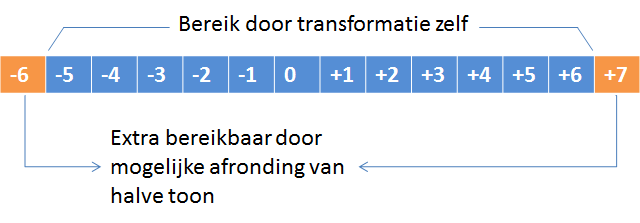
\includegraphics[width=0.75\textwidth]{4_Efficient_Toepassen_Transformatie/14}
  \caption{Illustratie van de 14 mogelijkheden om een noot in het muziekstuk te transformeren.}
  \label{figuur:14}
\end{figure}

Elke noot kan dus theoretisch gezien (na afronding) afgebeeld worden op eender welke noot die maximaal 6 halve tonen lager en maximaal 7 halve tonen hoger ligt dat zichzelf. Dit zijn in totaal 14 verschillende mogelijkheden.

\subsubsection{Hoog niveau idee van het algoritme}
Het belangrijkste idee van het algoritme is gebaseerd op de principes van \textit{dynamic programming} \cite{url:DP}. Toegepast op dit algoritme komt het er op neer dat achtereenvolgens voor elke noot in het muziekstuk het beste pad (en bijhorende beste score) bijgehouden zal worden voor elk van de 14 mogelijke toonhoogtes die deze noot kan aannemen in de nieuwe melodielijn. En enkel op deze optimale paden zal verder gerekend worden om te bepalen wat de beste paden zijn tot de 14 mogelijke toonhoogtes die de volgende noot in het muziekstuk kan aannemen. Dit wordt dan verder herhaald tot alle noten van de originele melodielijn overlopen zijn.

\subsection{Werking van het algoritme}
In dit onderdeel zal de werking van het algoritme beschreven worden. Als extra referentie voor de lezer is de broncode bijgevoegd in appendix \ref{Broncode:algo1}. Tijdens de uitvoer van het algoritme zal achtereenvolgens elke noot in het muziekstuk overlopen worden. Telkens zal voor elk van de noten waar de beschouwde noot naartoe getransformeerd kan worden enkel de probabiliteit bijgehouden worden van het pad dat eindigt op deze noot en het meest waarschijnlijk is.

\subsubsection{Notatie}
Voor het beschrijven van het algoritme worden een aantal notaties en functies beschreven. Allereerst wordt volgende notatie ingevoerd:

\begin{framed}
\noindent
$\mathcal{T}:$ Set van alle transformaties die beschikbaar zijn voor het algoritme, in deze set zit ook telkens de nultransformatie die een noot nooit verandert.\\
$\mathcal{P}:$ Set van alle noten waar de vorige beschouwde noot naartoe getransformeerd kan worden.\\
$\mathcal{C}:$ Set van alle noten waar de huidige noot naartoe getransformeerd kan worden.\\
$AN$: Het aantal noten in het muziekstuk.\\
$x$: Noot uit de originele melodielijn die beschouwd wordt als huidige noot in het algoritme.
\end{framed}

De functie $transform$ geeft weer dat een vorige noot $p\in \mathcal{P}$ de huidige noot $x$ in de originele melodie onder transformatie $t\in \mathcal{T}$ afbeeldt naar noot $c\in \mathcal{C}$.

\begin{framed}
\noindent
$transform(p,x,t)=c$
\end{framed}

De functie $proxProb$ geeft het logaritme terug van de probabiliteit gegeven door de \textit{proximity} parameter van het RPK-model. Als voor de overgang van noot $p\in \mathcal{P}$ naar noot $c\in \mathcal{C}$, de afstandsprobabiliteit tussen deze twee noten gelijk is aan $d$, dan geeft de functie $proxProb$ de volgende waarde terug

\begin{framed}
\noindent
$proxProb(p,c)=log(d)$
\end{framed}

De functie $posProb$ geeft het logaritme terug van de probabiliteit van een noot die enkel afhangt van de toonhoogte van de noot zelf. Deze probabiliteiten komen overeen met de \textit{range} en de \textit{key} parameters uit het RPK-model. Deze probabiliteit is dus onafhankelijk van de voorgaande noot. stel dat voor een noot $c\in \mathcal{C}$ de probabiliteit door de \textit{range} parameter gegeven wordt door $r$. Stel ook dat de probabiliteit bepaald door de \textit{key} gegeven wordt door $k$. Nu wordt de totale $posProb$ gegeven door:

\begin{framed}
\noindent
$posProb(c)=log(r) + log(k)$
\end{framed}

\subsubsection{Maximale probabiliteit}
$prob(c)$ geeft het logaritme van de probabiliteit weer van het meest waarschijnlijke pad dat eindigt op deze noot $c\in \mathcal{C}$.

Wanneer de eerste noot van het muziekstuk beschouwd wordt en $x$ dus de waarde heeft van deze eerste noot, zal de probabiliteit van het pad dat eindigt op deze noot gelijk zijn aan 1. De probabiliteit van alle andere noten is gelijk aan 0. Dit komt omdat de eerst noot van een muziekstuk nooit getransformeerd wordt. Aangezien het algoritme werkt met de logaritmen van deze probabiliteiten zullen de waarden respectievelijk op 0 en $-\infty$ gezet worden. Wanneer $x$ gelijk is aan de eerste noot van het originele muziekstuk geldt dus:

\begin{framed}
\noindent
$\forall c\in \mathcal{C}: \begin{cases} 
prob(c)=0 &\mbox{if } c==x\\ 
prob(c)=-\infty &\mbox{if } c!=x \end{cases}$
\end{framed}

Voor alle mogelijke noten op andere posities van het muziekstuk geldt dat:

\begin{framed}
\noindent
\begin{multline}
\forall c\in \mathcal{C}: 
prob(c) = max(prob(p) + proxProb(p,c) + posProb(c)) \\
| \forall p\in \mathcal{P}: \exists t\in \mathcal{T}: transform(p,x,t)=c
\end{multline}
\end{framed}

Door deze functie achtereenvolgens toe te passen voor alle noten van het muziekstuk kan er bepaald worden wat de probabiliteit is van het beste pad, gebruik makend van de gegeven transformaties uit $\mathcal{T}$. Dit zal namelijk gelijk zijn aan de hoogste probabiliteit van alle noten $c\in \mathcal{C}$ in de laatste stap van het algoritme.

\subsubsection{Optimale pad}
We zijn natuurlijk niet enkel ge\"interesseerd in de probabiliteit van het optimale pad, maar ook dit pad zelf, want dit gaat de gevonden melodie weergeven. Daarom wordt er voor de elke combinatie van een positie in de melodie en de mogelijke noten die op die positie kunnen voorkomen, bijgehouden waarvan het optimale pad kwam dat uitkwam bij die exacte noot op die positie. Om deze paden voor te stellen wordt de functie $path$ gebruikt. Meer algemeen, stel we zijn op positie $i$ in het algoritme (we beschouwen dus de $i$-de noot van het muziekstuk), dan zal wanneer het optimale pad dat eindigt op noot $n$ komt van een zekere $m$, het volgende gelden:

\begin{framed}
\noindent
$path(i,n)=m$
\end{framed}

Wanneer het algoritme voor alle mogelijke noten op elke positie in de melodie de maximale probabiliteit bepaald heeft kan het optimale pad gevonden worden. Dit gebeurt zoals beschreven in algoritme \ref{alg:opt_pad}.

\begin{algorithm}
\caption{Optimaal pad}\label{alg:opt_pad}
\begin{algorithmic}
\State $note=argmax_{c \in \mathcal{C}}(prob(c))$
\State $Path.addToFront(note)$
\For {($i = AN: i\geq 2: i=i-1$)}{}	
	\State $note = path(i,note)$
	\State $Path.addToFront(note)$
\EndFor
\State \Return $Path$
\end{algorithmic}
\end{algorithm}

Intern in het algoritme worden al deze $path$ relaties opgeslagen in een $(n\times 14)$-\textit{matrix}. voor elk van de $n$ posities in de melodie worden voor alle 14 noten waar theoretisch naar getransformeerd kan worden, de index bijgehouden van de noot op de vorige positie waarvan het optimale pad kwam. Een voorbeeld van hoe hier een pad uit gereconstrueerd kan worden, is afgebeeld in figuur \ref{figuur:matrix}. Voor twee verschillende noten op positie $i$ in het muziekstuk wordt het optimale pad om tot die noot te geraken afgebeeld. De waarden die in de vakjes staan zijn telkens indexen die verwijzen naar een noot op de vorige positie.

\begin{figure}[!ht]
  \centering
  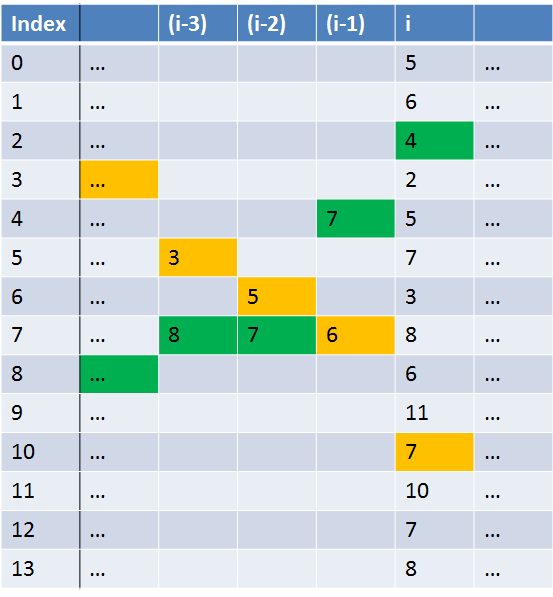
\includegraphics[width=0.75\textwidth]{4_Efficient_Toepassen_Transformatie/matrix}
  \caption{Illustratie van de reconstructie van het optimale pad voor 2 verschillende noten op positie $i$.}
  \label{figuur:matrix}
\end{figure}

\subsection{Performantie en geheugencomplexiteit}
De eerste parameter waarvan het algoritme afhankelijk is, is de lengte van de melodielijn of met andere woorden het aantal noten (AN) in de invoer. Ook het aantal beschikbare transformaties (AT) heeft een invloed (in het voorbeeld beschreven in appendix \ref{Broncode:algo1} wordt gebruik gemaakt van slechts 2 transformaties, maar het algoritme werkt voor eender welk aantal transformaties dat gedefinieerd wordt).

\subsubsection{Tijd} 
De snelheid van het algoritme is lineair afhankelijk van beide van deze parameters. Indien de lengte van het originele melodietje met een factor $f$ omhoog gaat en de rest constant blijft dan gaat ook het aantal stappen in het algoritme met een factor $f$ omhoog. Het rekenwerk per stap blijft echter gelijk. Wanneer het aantal transformaties met een factor $t$ omhoog gaat en de rest constant blijft, dan zal het aantal stappen onveranderd blijven. Het rekenwerk per stap gaat wel met een factor $t$ omhoog (op het constante rekenwerk per stap van het `niet transformeren' na).

\begin{center}
\underline{Tijd:} $\mathcal{O}(AN \times AT)$
\end{center}

\subsubsection{Geheugen}
De hoeveelheid geheugen die nodig is voor de uitvoer van het algoritme is lineair afhankelijk van de lengte van de originele melodie. Dit komt omdat de \textit{matrix} array als een van zijn dimensies deze lengte heeft. Wanneer de lengte van het originele stukje met een factor $f$ omhoog gaat, zal de grootte van deze array dus ook met een factor $f$ omhoog gaan. De grootte van de andere twee gebruikte arrays(\textit{past} en \textit{current}) is onveranderlijk ten opzichte van die lengte. De transformaties zelf moeten natuurlijk ook opgeslagen worden, waardoor de het geheugengebruik ook lineair afhankelijk is van het aantal transformaties. maar in het totale geheugengebruik is de \textit{matrix}-array dominant en opzichte van de opslag van de respresentaties van de transformaties, aangezien deze zo veel groter is. Het aantal gebruikte transformaties heeft dus weinig effect op het geheugengebruik van het algoritme. En in het algemeen kan er dus veronderstel worden dan het aantal gebruikte transformaties het geheugengebruik niet merkbaar be\"invloedt.

\begin{center}
\underline{Geheugen:} $\mathcal{O}(AN)$
\end{center}

\section{Beste sequentie met minimum transformatie lengte}
\label{ETT:algo2}

\subsection{Doelstelling}
Het algoritme dat in dit onderdeel beschreven wordt heeft dezelfde doelstelling als het algoritme beschreven in onderdeel \ref{ETT:algo1}. Enkel wordt dit algoritme aan nog een extra restrictie onderworpen.

Zo zal dit algoritme afhankelijk zijn van drie parameters. De eerste twee parameters zijn een originele melodielijn en een aantal toegelaten transformaties. Als extra parameter is dit algoritme nog afhankelijk van een opgegeven minimum transformatie lengte.

Dit betekent dat het algoritme enkel een deel van de originele melodielijn mag transformeren als het voor minstens dit opgegeven aantal opeenvolgende noten dezelfde transformatie uitvoert.

\subsection{Idee van het algoritme}
\subsubsection{Hoog niveau idee van het algoritme en notatie}
Ook nu zal er gebruik gemaakt worden van de principes van \textit{dynamic programming}. Dit zal enkel op een verschillende manier gebeuren dan bij het vorige algoritme, aangezien de opgegeven minimumlengte verhindert om eenzelfde data representatie te gebruiken. Ook zullen dezelfde regels gelden als in het overeenkomstige onderdeel uit \ref{ETT:algo1} wat het bereik van een tranformatie betreft.

Het idee van het algoritme bestaat erin om elke noot van het muziekstukje chronologisch te overlopen. Bij elke noot uit het originele stuk zijn er dan een aantal mogelijkheden om het beste pad te bepalen dat eindigt op een van de 14 mogelijke noten waarnaar de originele noot getransformeerd kan worden.
 
Als in het vervolg van de tekst gesproken wordt over een ``geldig pad'', dan wordt hier een pad mee bedoeld dat de regels van de minimumlengte voor transformatie respecteert.

\subsubsection{Verschillende mogelijkheden om tot een optimaal pad te komen} 
In dit onderdeel wordt een intu\"itieve beschrijving gegeven van hoe het optimale pad tot op een bepaalde positie in het muziekstuk kan berekend worden. Dit, gebruik makend van de optimale paden en bijhorende probabiliteiten van de noten op vorige posities in het muziekstuk.

Een eerste mogelijkheid voor een optimaal pad is de uitbreiding van eender welk optimaal pad dat eindigt op een van de noten waar de vorige noot uit het muziekstuk naar getransformeerd kan worden.
 
Een tweede mogelijkheid is het uitbreiden van een optimaal pad dat geldig is, eindigt op de vorige noot en eindigt met transformatie f uit te breiden met dezelfde transformatie f.
 
Tot slot is er ook nog de mogelijkheid om eender welk optimaal en geldig pad dat een lengte ML korter is dan het huidige uit te breiden met ML keer dezelfde transformatie. Op deze manier kunnen alle optimale paden bekomen worden die aan de vooropgestelde eisen voldoen.

\subsection{Werking van het algoritme}
In dit onderdeel zal de werking van het algoritme beschreven worden. Als extra referentie voor de lezer is de broncode bijgevoegd in appendix \ref{Broncode:algo2}. Tijdens de uitvoer van het algoritme zal achtereenvolgens elke noot in het muziekstuk overlopen worden. Nu zal voor elke transformatie apart bijgehouden worden wat de optimale paden en probabiliteiten zijn voor alle verschillende noten waar de huidige noot naartoe getransformeerd kan worden en die eindigen met die specifieke transformatie. 

\subsubsection{Notatie}
Voor het beschrijven van het algoritme worden een aantal notaties en functies beschreven. Allereerst wordt volgende notatie ingevoerd:

\begin{framed}
\noindent
$\mathcal{T}:$ Set van alle transformaties die beschikbaar zijn voor het algoritme, in deze set zit ook telkens de nultransformatie die een noot nooit verandert.\\
$nt$: De nultransformatie die ook in $\mathcal{T}$ zit.\\
$ML$: De minimum transformatie lengte.\\
$\mathcal{P_{ML}}:$ Set van alle noten waar de noot die $ML$ posities voor de huidige noot naartoe getransformeerd kan worden.\\
$\mathcal{P}:$ Set van alle noten waar de vorige beschouwde noot naartoe getransformeerd kan worden.\\
$\mathcal{C}:$ Set van alle noten waar de huidige noot naartoe getransformeerd kan worden.\\
$AN$: Het aantal noten in het muziekstuk.\\
$x$: Noot uit de originele melodielijn die beschouwd wordt als huidige noot in het algoritme.\\
$i$: De index van de noot die momenteel beschouwd wordt in het algoritme.\\
$OL$: Geordende lijst van de noten in de originele melodie.
\end{framed}

De functie $transform$ geeft weer dat een vorige noot $p\in \mathcal{P}$ de huidige noot $x$ in de originele melodie onder transformatie $t\in \mathcal{T}$ afbeeldt naar noot $c\in \mathcal{C}$.

\begin{framed}
\noindent
$transform(p,x,t)=c$
\end{framed}

De functie $proxProb$ geeft het logaritme terug van de probabiliteit gegeven door de \textit{proximity} parameter van het RPK-model. Als voor de overgang van noot $p\in \mathcal{P}$ naar noot $c\in \mathcal{C}$, de afstandsprobabiliteit tussen deze twee noten gelijk is aan $d$, dan geeft de functie $proxProb$ de volgende waarde terug

\begin{framed}
\noindent
$proxProb(p,c)=log(d)$
\end{framed}

De functie $posProb$ geeft het logaritme terug van de probabiliteit van een noot die enkel afhangt van de toonhoogte van de noot zelf. Deze probabiliteiten komen overeen met de \textit{range} en de \textit{key} parameters uit het RPK-model. Deze probabiliteit is dus onafhankelijk van de voorgaande noot. stel dat voor een noot $c\in \mathcal{C}$ de probabiliteit door de \textit{range} parameter gegeven wordt door $r$. Stel ook dat de probabiliteit bepaald door de \textit{key} gegeven wordt door $k$. Nu wordt de totale $posProb$ gegeven door:

\begin{framed}
\noindent
$posProb(c)=log(r) + log(k)$
\end{framed}

Tot slot is er ook nog een algoritme $extendPath$ dat berekent wat het logaritme van de probabiliteit is van de uitbreiding van een pad. Deze uitbreiding moet van lengte $l$ zijn en volgens een meegegeven transformatie $t\in \mathcal{T}$ bekomen worden. Dit algoritme krijgt ook het pad $path$ waarop deze uitbreiding moet uitgevoerd worden mee. Tot slot wordt aan dit algoritme wordt ook een lijst $list$ van opeenvolgende noten meegegeven, dit zijn de noten van het originele muziekstuk waarop deze transformatie toegepast moet worden. Dit algoritme geeft niet alleen het logaritme van de probabiliteit van deze uitbreiding mee, maar ook het volledige pad dat na uitbreiding bekomen wordt.

\begin{algorithm}
\caption{$extendPath(l,t,Path,list)$}\label{alg:opt_pad}
\begin{algorithmic}
\State $Prob = 0$
\State $p$ = $Path.last$
\For {($i = 1: i \leq l: i=i+1$)}{}	
	\State $x = list[i]$
	\State $c = transform(p,x,t)$
	\State $Path.add(c)$
	\State $Prob = Prob + proxProb(p,c) + posProb(c)$
	\State $p = c$
\EndFor
\State \Return $(Prob, Path)$ 
\end{algorithmic}
\end{algorithm}

\subsubsection{Optimale paden voor verschillende transformaties}
De reden dat paden die eindigen op verschillende transformaties apart bijgehouden worden heeft twee redenen. 

Ten eerste zal, wanneer het algoritme op voorhand weet dat een bepaald pad geldig is (voldoet aan de voorwaarden voor minimum transformatie lengte) en eindigt op een zeker transformatie $t$, weten dat dit pad enkel door dezelfde transformatie $t$ kan uitgebreid worden naar enkel de volgende noot. Voor andere transformaties zal minstens $ML$ keer die transformatie moeten toegepast worden. Met deze voorstelling is het meteen duidelijk welke transformatie ook voor een noot mag uitgevoerd worden en welke voor minstens $ML$ volgende noten moet uitgevoerd worden om terug een geldig pad te bekomen.

Ten tweede heeft het ook te maken met de extra eis van de minimum transformatie lengte. Indien alle optimale paden zouden bijgehouden worden met een $path$ relatie zoals in het vorige algoritme, die onafhankelijk zou zijn van de transformatie waarop ge\"eindigd werd, dan kan tijdens de uitvoer van het algoritme de regel van de minimum transformatie lengte geschonden worden. Een voorbeeld hiervan wordt hieronder gegeven:

\begin{framed}
\noindent
Stel dat:
$ML=2$\\
$path(3,W_1) = V_1$\\
$path(2,V_1) = U_1$\\
$path(3,W_2) = V_2$\\
$path(2,V_2) = U_2$\\
Dan zijn momenteel de optimale paden voor $W_1$ en $W_2$, respectievelijk $U_1-V_1-W_1$ en $U_2-V_2-W_2$.\\
Stel verder dat het optimale pad voor $W_1$ bekomen werd door tweemaal een transformatie $t_1 \in \mathcal{T}$ toe te passen en dat het optimale pad voor $W_2$ bekomen werd door tweemaal $t_2 \in \mathcal{T}$ toe te passen.\\
Beide paden zijn momenteel dus geldig onder de voorwaarde van de minimum transformatie lengte.\\
Stel nu dat er in het verdere verloop van het algoritme nog een beter pad gevonden wordt dat eindigt in $W_2$ en dat verloopt volgens $U_2-V_1-W_2$. Stel ook dat dit pad gevonden werd door het tweemaal toepassen van $t_3 \in \mathcal{T}$. Nu wordt de $path$ functie aangepast zodat deze de juiste waarden teruggeeft.\\
Nu geldt:\\
$path(3,W_1) = V_1$\\
$path(2,V_1) = U_2$\\
$path(3,W_2) = V_1$\\
$path(2,V_2) = U_2$\\
Dan zijn nu de optimale paden voor $W_1$ en $W_2$, respectievelijk $U_2-V_1-W_1$ en $U_2-V_1-W_2$.\\
Het optimale pad van $W_1$ is nu geen geldig optimaal pad meer aangezien het door het achtereenvolgens toepassen van telkens een maal de transformatie $t3$ en $t1$ niet meer voldoet aan de voorwaarden van de minimum transformatie lengte.
\end{framed}

\subsubsection{Maximale probabiliteit}
$prob(c,t)$ geeft het logaritme van de probabiliteit weer van het meest waarschijnlijke pad dat eindigt op deze noot $c\in \mathcal{C}$. Deze noot (en zelfs minstens de laatste $ML$ noten) moet in dit geval bekomen zijn door gebruik van transformatie $t \in \mathcal{T}$.

Wanneer de eerste noot van het muziekstuk beschouwd wordt en $x$ dus de waarde heeft van deze eerste noot, zal de probabiliteit van het pad dat eindigt op deze noot gelijk zijn aan 1. De probabiliteit van alle andere noten is gelijk aan 0. Dit komt omdat de eerste noot van een muziekstuk nooit getransformeerd wordt. Dit zal enkel het geval zijn voor de nultransformatie. Voor alle andere transformaties zal eender welke noot een kans 0 hebben om deel uit te maken van het optimale pad aangezien er geen enkel optimaal pad kan zijn dat eindigt op een transformatie als dat pad maar een noot kan bevatten. Aangezien het algoritme werkt met de logaritmen van deze probabiliteiten zullen de waarden respectievelijk op 0 en $-\infty$ gezet worden. Wanneer $x$ gelijk is aan de eerste noot van het originele muziekstuk en transformatie $t\in \mathcal{T}$ beschouwd wordt geldt dan:

\begin{framed}
\noindent
$\forall c\in \mathcal{C}, t\in \mathcal{T} \begin{cases} 
prob(c,t)=0 &\mbox{if } c==x $ \& $ t=nt\\ 
prob(c,t)=-\infty &\mbox{if } c==x $ \& $ t!=nt\\ 
prob(c,t)=-\infty &\mbox{if } c!=x \end{cases}$
\end{framed}

Voor alle andere noten en transformaties op alle andere posities in het muziekstuk geldt:

\begin{framed}
\noindent
\begin{multline}
\forall t\in \mathcal{T}: 
ProbSame(c,t) = max(prob(p,t) \\ 
+ extendPath(1,t,path(i-1,p,t),OL[i]).prob) \\
| \forall p\in \mathcal{P}: transform(p,x,t)=c
\end{multline}

\begin{multline}
\forall t\in \mathcal{T}: 
ProbDifferent(c,t) = max(prob(p_{ML},t) \\ 
+ extendPath(i-ML,t,path(i-ML,p_{ML},t1).prob,OL[(i-ML+1)..i]) \\
| \forall p_{ML}\in \mathcal{P_{ML}}, \forall t1\in \mathcal{T}:\\
t1!=t, extendPath(i-ML,t,path(i-ML,p_{ML},t1).path.last=c
\end{multline}

\begin{multline}
\forall c\in \mathcal{C}, t\in \mathcal{T}: 
prob(c,t) = max(ProbSame(c,t), ProbDifferent(c,t))
\end{multline}
\end{framed}

Door deze functie achtereenvolgens toe te passen voor alle noten van het muziekstuk kan er bepaald worden wat de probabiliteit is van het beste pad, gebruik makend van de gegeven transformaties uit $\mathcal{T}$ rekening houdend met de minimum transformatie lengte $ML$. Dit zal namelijk gelijk zijn aan de hoogste probabiliteit van de combinatie van alle noten $c\in \mathcal{C}$ en transformaties $t\in \mathcal{T}$ in de laatste stap van het algoritme.

\subsubsection{Optimale pad}
$path(i,n,t)$ stelt het volledige pad voor dat optimaal is onder de gegeven voorwaarden en dat eindigt bij noot $n$ op positie $i$ en door te eindigen met transformatie $t\in \mathcal{T}$. Initieel zijn al deze paden volledig leeg, enkel het pad dat eindigt op de nultransformatie en op de noot die gelijk is aan de startnoot bestaat uit exact deze noot. Telkens er een pad gevonden wordt dat eindigt op  noot $n$ en met transformatie $t\in \mathcal{T}$, dan zal niet enkel de $prob(n,t)$ waarde aangepast worden, maar ook $path(i,n,t)$ zal het nieuwe beste pad bevatten voor de combinatie van deze parameters.

Aangezien volledige beste paden bijgehouden worden moet er geen werk verricht worden om het beste pad te bepalen. Er moet enkel dat pad gekozen worden van lengte $AN$ dat de hoogste probabiliteit oplevert. Voor de combinatie van alle noten $c\in \mathcal{C}$ en transformaties $t\in \mathcal{T}$ is er zo een optimaal pad dat hier een kandidaat voor is. Van al deze kandidaten zal het pad met de hoogste probabiliteit het optimale pad zijn voor het geheel.

\begin{framed}
\noindent
$optPath=argmax_{c\in \mathcal{C}, t\in \mathcal{T}}(prob(path(AN,c,t)))$
\end{framed}

\subsection{Performantie en geheugencomplexiteit}
In dit algoritme zijn er drie parameters waar rekening mee dient gehouden te worden bij het bespreken van de tijds- en geheugencomplexiteit. Deze drie parameters zijn het aantal noten in de originele melodielijn (AN), het aantal beschikbare transformaties (AT) en de minimum transformatie lengte (ML).

\subsubsection{Tijd}
De performantie van het algoritme is lineair afhankelijk van het aantal noten. Dit komt doordat voor elke noot in het oorspronkelijk muziekstuk een stap in het algoritme moet uitgevoerd worden. Het rekenwerk per stap verandert niet wanneer de lengte van het stuk verandert.
 
De snelheid van het algoritme is kwadratisch afhankelijk van het aantal toegestane transformaties. Dit komt omdat voor elke stap in het algoritme we voor elke transformatie gaan proberen een optimaal pad te vinden dat kan vertrekken van bij tussenoplossingen horende bij alle andere transformaties. Het aantal stappen in het algoritme verandert niet wanneer het aantal transformaties verandert. In totaal geeft dit dus een kwadratische afhankelijkheid.

Tot slot is de snelheid van het algoritme ook afhankelijk van de minimum transformatie lengte volgens $\mathcal{O}(ML \times (AN-ML))$. zowel het aantal stappen in het algoritme als het aantal berekende paden per stap zal onveranderd blijven wanneer deze parameter verandert. Het extra rekenwerk dat gecre\"eerd wordt door het moeten uitbreiden van paden die $ML$ korter zijn dan de huidige lengte is lineair afhankelijk van de grootte van $ML$. Maar het aantal paden dat zo berekend moet worden is lineair afhankelijk van $(AN-ML)$. Hierdoor zal de totale rekentijd afhankelijk zijn van het product van deze twee.

\begin{center}
\underline{Tijd:} $\mathcal{O}(AN \times ML \times (AN-ML) \times AT^2)$
\end{center}

\subsubsection{Geheugen}
De totale opslagcapaciteit die noodzakelijk is voor de uitvoer van het algoritme is ten eerste lineair afhankelijk van de lengte van de invoer sequentie van noten. Voor alle mogelijke transformaties zullen namelijk optimale paden bijgehouden worden en de lengte van deze paden is altijd van dezelfde grootte-orde als de lengte van het originele.

Ten tweede is het geheugengebruik ook lineair afhankelijk van de minimum transformatie lengte. Er worden namelijk optimale sub paden bijgehouden in het algoritme voor de laatste $ML$ beschouwde noten. De lengte van deze paden is ook elk van dezelfde grootte-orde.
 
Tot slot is er nog het aantal transformaties. Ook deze parameter zal een lineaire invloed hebben op het geheugengebruik. Dit aangezien voor elke beschikbare transformatie even veel optimale paden bijgehouden worden die eindigen op deze transformatie.  

\begin{center}
\underline{Geheugen:} $\mathcal{O}(AN \times ML \times AT)$
\end{center}

%%% Local Variables: 
%%% mode: latex
%%% TeX-master: "masterproef"
%%% End: 
